\startchapter{Simplified Molecular Model} \label{ch:3}

\section{Description}
The goal of Chapter \ref{ch:3} is to further expand the research focus and introduce the formulas used to generate the LP models. Before studying real life molecules, first a toy molecule with limited vibration modes is studied. By doing so, the nature of the LP formulas used to gain some further insights of the models built is carefully analyzed. The goal is to figure out with the all the available spectral information, could LP models built output any valuable information. If the LP models have limitation in achieving this goal, then the reason behind needed to further explained. \\

%In the last chapter, we have seen how IR, Raman and SFG spectres are produced theoretically. However, before we jump to the real molecule models, we would like to study the further properties of our LP model first: with the data information we have, can our LP model give us some valuable information? Moreover, which data collection method from different spectra techniques can be more valuable when combining LP? Those two questions are the targets we want to aim on.

A toy molecule with $4$ vibration modes is constructed. Theses vibrational peaks are at frequencies of $2850, 2960, 3050$ and $3200$. The width of the peak are $5, 10, 5$ and $15$ respectively. The amplitude of the peak are $1, 0.7, -0.2$ and $0.5$, respectively. The comparing angles of the peak is $15, 90, 0$ and $60$. (TODO: check with Dennis, how to explain those comparing angles?)  \\

For this toy model, only IR spectroscopy is considered. Equation \ref{eq:3.1} is used to generate the cosine projection IR spectroscopy. Moreover, Only the difference on $\theta$ angle is considered. \\

\begin{eqnarray} \label{eq:3.1}
& f_{\theta}(x) = \displaystyle\sum^{4}_{q=1} A_q^2 * cos^2(\theta - \theta_q)\frac{\gamma^2}{(x- w_q)^2 + \gamma^2} 
\end{eqnarray}

where $A$ is the amplitude, $theta_{q}$ is the $tilt$ angle of the candidate, $\gamma$ is the width, $w_q$ is the frequency. (TODO: Double check the correct meaning of each symbol) $10$ different candidates' with 10 different $\theta$ values as followed: $0^{\circ}$, $10^{\circ}$, $20^{\circ}$, $30^{\circ}$, $40^{\circ}$, $50^{\circ}$, $60^{\circ}$, $70^{\circ}$, $80^{\circ}$, $90^{\circ}$. Their spectra are generated as shown in Figure \ref{fig:3.1}. The 10 candidates have peaks at the same frequencies. The spectral signal for candidates is comparatively strong at each peak, and distinguish each candidate more than other signal. \\

%However, one may wonder that the spectrum among all the candidates here may look quite similar to each other. This does not matter much in appearance, however, may make it difficult to obtain the exact composition for the targeted spectrum, as various combinations of candidates are possible to achieve the targeted spectrum. We will need to run certain experiments to further demonstrate this point. \\

%This is the cosine projection of the IR spectra. Furthermore, this molecule only contains 4 vibration modes, with the peaks happen at frequency of 2850, 2960, 3050 and 3200, and the widths for the peaks are 5, 10, 5 and 15, and the heights, which are 1, 0.7, -0.2 and 0.5 respectively. The comparing angle for each peak( What does those angle refer???) is 15, 90, 0 and 60. We generate 10 candidate spectra with 10 different $\theta$ values: $\theta = 0^{\circ}, 10^{\circ}, 20^{\circ}, 30^{\circ}, 40^{\circ}, 50^{\circ}, 60^{\circ}, 70^{\circ}, 80^{\circ}, 90^{\circ} $ \\

\begin{figure}[!ht] \label{fig:3.1}
\centering
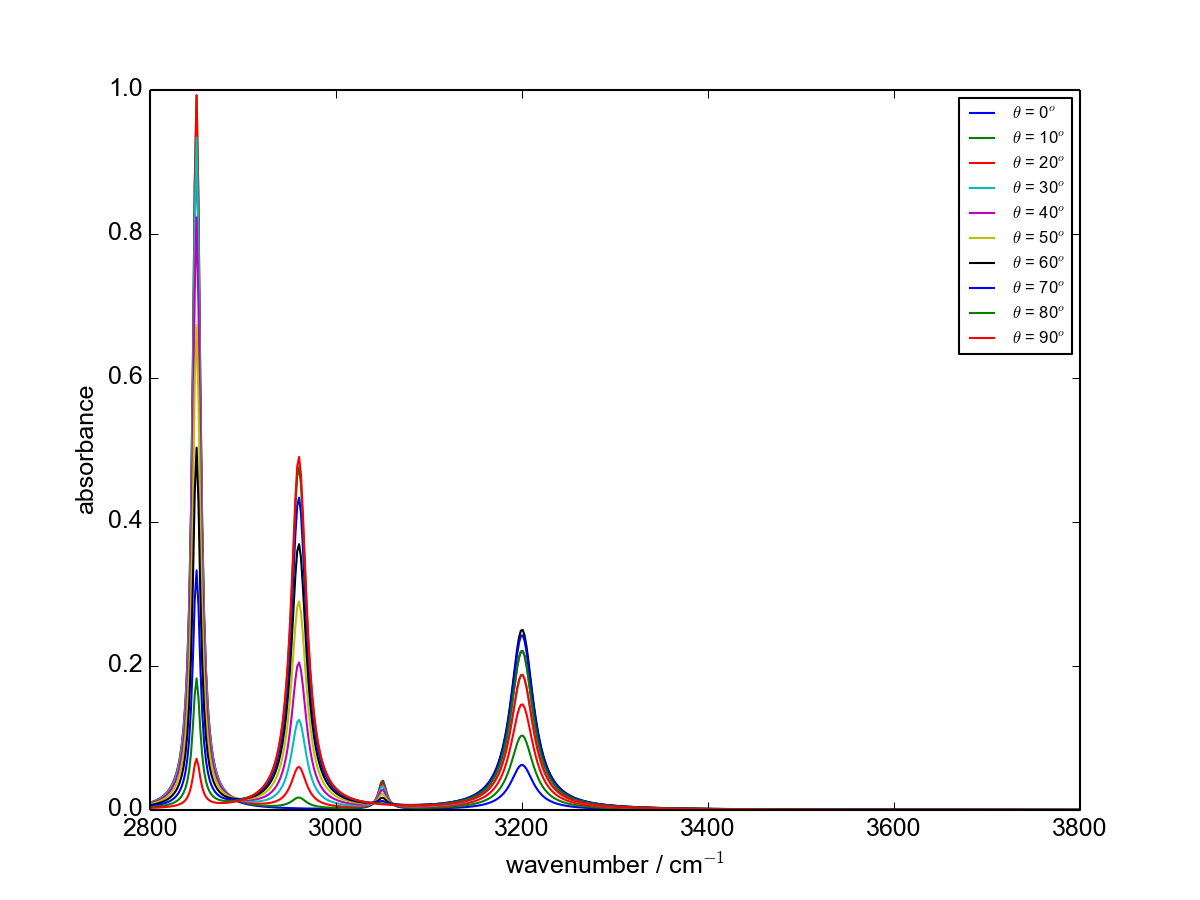
\includegraphics[scale=0.4]{Figures/Toy_Model_IR_Cosine_Projection.png} 
\caption{Toy model IR candidates cosine projection} 
\end{figure}

A target spectrum is composed by combining $15$ percent of candidate with $\theta$ of $20^{\circ}$ and $85$ percent of candidate of $\theta$ of $70^{\circ}$: $0.15*f_{20}(x) + 0.85*f_{70}(x)$ in the following experiment. \\

\section{Linear Programming Model for Spectra Study}

The LP model constructed to check if the optimal solution returned by the LP solver actually matches to the known composition is shown in Equation \ref{eq:3.2}. This model has also been used to study the composition analysis of Ribonucleic acid (RNA) with ultraviolet (UV) spectra and other UV spectroscopy studies back in 60s \cite{NYAS:NYAS900} \cite{LPATUAS}. \\

\begin{eqnarray} \label{eq:3.2}
& minimize \displaystyle\sum^{points}_{p=1} \left| Target- \displaystyle\sum^{candidates}_{c=1}p_{c}f_{\theta}(x) \right| 
\end{eqnarray}
where $p_{c}$ is the unknown percentage of each candidate, which is the decision variable. $p$ is the number of points selected along the wavenumber, both from candidates and target spectra. For each data point, the absolute residual between target spectrum and the one composed by the decision variables is calculated. The objective function minimizes the sum of the absolute residuals over all the data points. \\

However, in order to apply LP, getting rid of the absolute signs in the objective function is needed. Because Equation \ref{eq:3.2} subject to no restrictions, meanwhile, the objection function is not in standard form. This is achieved by introducing one more variable $X$ and two more constraints for each data point as shown in Equation \ref{eq:3.3}. Then the previous model in Equation \ref{eq:3.2} is converted into Equation \ref{eq:3.4}, which can actually be solved by LP solver. At last, one more constraint is introduced to restrict the sum of the percentages to be 1, as shown in Equation \ref{eq:3.4}. \\

For each point:
\begin{eqnarray} \label{eq:3.3}
& X = \left| Target-\displaystyle\sum^{candidates}_{c=1}p_{c}f_{\theta}(x) \right| \nonumber \\
&  X \geq Target-\displaystyle\sum^{candidates}_{c=1}p_{c}f_{\theta}(x)   \nonumber \\
& X \geq -Target+\displaystyle\sum^{candidates}_{c=1}p_{c}f_{\theta}(x)  
\end{eqnarray} 

\begin{eqnarray} \label{eq:3.4}
& minimize \displaystyle\sum^{points}_{p=1} X_p \nonumber \\
& X_1 - Target_1 + \displaystyle\sum^{candidates}_{c=1}p_{c}f_{\theta}(x_1) \geq 0 \nonumber \\
& X_1 + Target_1 - \displaystyle\sum^{candidates}_{c=1}p_{c}f_{\theta}(x_1) \geq 0 \nonumber \\
& ... \nonumber \\
& X_n - Target_n + \displaystyle\sum^{candidates}_{c=1}p_{c}f_{\theta}(x_n) \geq 0 \nonumber \\
& X_n + Target_n - \displaystyle\sum^{candidates}_{c=1}p_{c}f_{\theta}(x_n) \geq 0 \nonumber \\
& \displaystyle\sum^{candidates}_{c=1}p_{c} = 1 
\end{eqnarray} 

\section{Linear programming model implementation}

To start, code is written to generate a file that contains all the candidates' spectral information needed for the experiments. For this step, the molecular properties in the pickle files are used. For a specific candidate, given the molecular propterties and the $\theta$ value, the candidate's spectral information is obtained. \\

In the first step, a candidate class is written. This class defines candidate's $x$- and $z$- polarized IR spectra; $xx$-, $xy$-, $xz$-, and $zz$- projection Raman spectra; $yyz$-, $yzy$-, $zzz$- projection SFG spectra. Given candidate's molecular properties and $\theta$ value, a instance of this specific candidate is created. For the toy model, it only contains IR spectral information. Therefore, one candidate only contains $cosine$- and $sine$- polarized IR spectra. \\

%In first step, I create a class that called Candidate in $candidate\_class.py$. This class defines one candidate's $x$- and $z$- polarized IR spectrum; $xx$-, $xy$-, $xz$-, and $zz$- projection Raman spectrum; $yyz$-, $yzy$-, $zzz$- projection SFG spectrum. Given one candidate's pickle file and $\theta$ value, $candidate\_class.py$ will create a instance of this specfic candidate. For the toy model, it only contains IR spectral information, therefore, one candidate only contains $cosine$- and $sine$- polarized IR spectrum. \\
%$create\_candidates.py$

In the second step, more code is written to generate a target composition of a list of needed candidates. Then the target composition is used to generate the target spectra. The probe arrange, which is the range of the wavenumber, is from 2800 to 3300. For further experiments in Chapter \ref{ch:4}, \ref{ch:5} and \ref{ch:6}, the probe arrange is from 2000 to 3000 wavenumber. Then all the spectral information of candidates and target is create in a text file. The code can also be used to run experiments that contain different spectroscopy information. For example, one file can contain only candidates and target's IR spectral information, or contain all three spectroscopy information. \\

In the third step, LP model is constructed by using the text file. This part of the code is written by Kai \cite{KuoKaiHung:Thesis:2015}. It reads all the candidates and target spectral information, and builds the LP model as shown in Equation \ref{eq:3.4}, then creates CPLEX LP input file. \\

In the fourth step, use LP solver to obtain the result. \\

\section{Experiments}
To further simplify the problem, in the first experiment set, it is necessary to limit the candidate numbers to be $4$. Table \ref{tab:3.1} illustrates the detailed settings for Experiment 1 and 2. In the first experiment, there are $4$ candidates with $\theta$ of $0^{\circ}, 10^{\circ}, 20^{\circ}$, and $30^{\circ}$. In the second experiment, the $\theta$ values are changed to $0^{\circ}, 5^{\circ}, 10^{\circ}$, and $15^{\circ}$. Instead of having a $10$ degree variance in the $\theta$, $5$ degree difference is applied on $\theta$. This means that the candidates become slightly more similar to each other, their spectra become more similar as well. The increase in similarity results in the problem more difficult to resolve. In both experiments, 100 data points are selected evenly along the wavenumber from the spectra of $cosine$-polarized IR. The target composition of the candidates are the same for both experiments. In Experiment 1, the return composition is the same as the target one, however, the return composition for Experiment 2 does not match to the target one. 

\begin{table} \label{tab:3.1}
\begin{center}
\begin{tabular}{| l | l | l | }
\hline
Experiment index & 1 & 2  \\
\hline
Number of Candidates & 4 & 4  \\
\hline
Candidates & [0, 10, 20, 30] & [0, 5, 10, 15] \\
\hline
Target Composition & [0.1, 0.5, 0.4, 0] & [0.1, 0.5, 0.4, 0]     \\
\hline
Number of Data Points & 100(cos) &  100(cos)     \\
\hline
Return Composition & [0.1, 0.5, 0.4, 0] & [0, 0.796962, 0.103038, 0.1] \\
\hline
\end{tabular} 
\end{center}
\caption{Experiment 1 and 2 Setting}
\end{table}	

%With the LP model we introduced in last section, we plotted the data of the first experiment to the model, and we got the result that was the same as the target composition. Right now, let's have a look at the second experiment, the only difference is that we changed the candidates a little bit, instead of having 10 degree variance in the theta, we have 5 degree difference on theta. This means that the candidates were becoming more and more similar, their spectra were getting similar to each other as well, which made the problem even more difficult to resolve. 

In order to figure out why the return composition in Experiment 2 is different from the target one, the spectra generated by the return composition is plotted together with the target spectra as shown in Figure \ref{fig:3.2}. Interesting thing is that these two spectrum are almost identical to each other. In order to see whether it is the general case, another experiment is set up in Table \ref{tab:3.2}. This experiment is slightly more complex than Experiment 1 and 2. There are $10$ candidates, including the $\theta$ values ranging from $0^{\circ}$ to $90^{\circ}$.  \\

\begin{figure}[!ht] \label{fig:3.2}
\centering
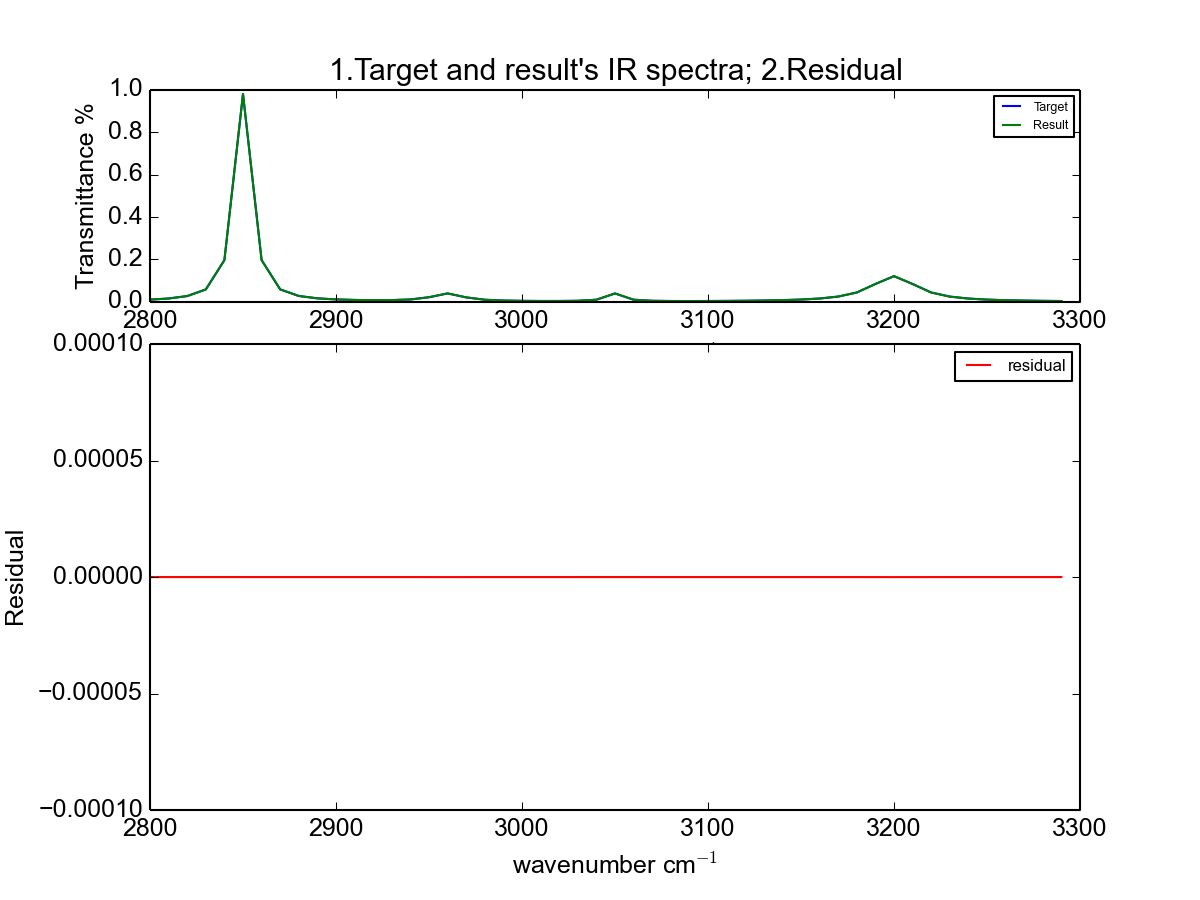
\includegraphics[scale=0.3]{Figures/toy_model_result_plotting_ir_cos_4candi_1.png}
\caption{Toy Model Result Plotting for 4 Candidates on IR Cosine Projection}
\end{figure}

\begin{table} \label{tab:3.2}
\begin{center}
\begin{tabular}{| l | p{7cm} | }
\hline
Experiment index & 3  \\
\hline
Number of Candidates & 10   \\
\hline
Candidates & [0, 10, 20, 30, 40, 50, 60, 70, 80, 90]  \\
\hline
Target Composition & [0.1, 0, 0.5, 0, 0.4, 0, 0, 0, 0, 0] \\
\hline
Number of Data Points & 100(cos) \\
\hline
Return Composition & [0, 0, 0.730541, 0, 0.212061,0, 0, 0.0573978, 0, 0] \\
\hline
\end{tabular}
\end{center}
\caption{Experiment 3 Setting}
\end{table}	

\begin{figure}[!ht] \label{fig:3.3}
\centering
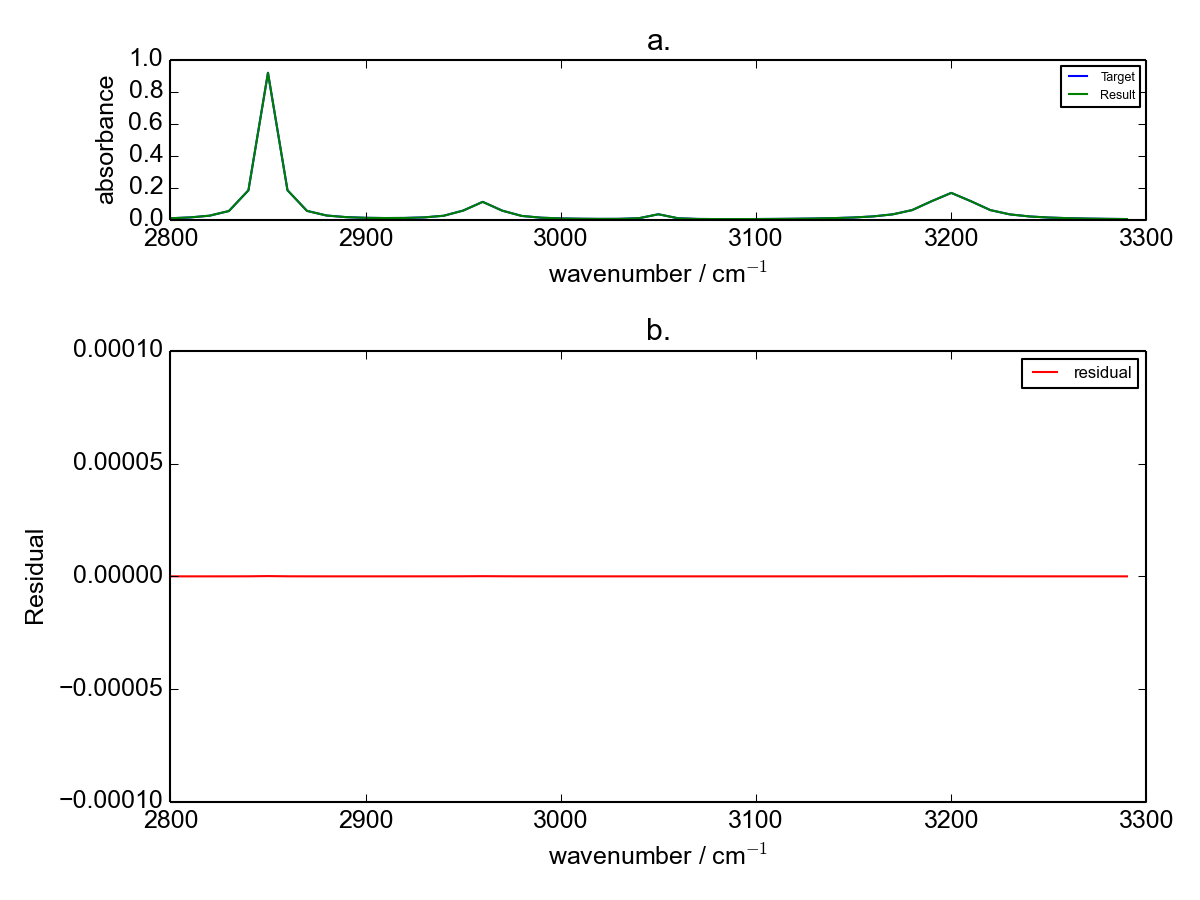
\includegraphics[scale=0.3]{Figures/toy_model_result_plotting_ir_cos_10candi_1.png} 
\caption{Toy Model Result Plotting for 10 Candidates on IR Cosine Projection}
\end{figure}

It can be seen in Table \ref{tab:3.2} that: the return composition is different from the target one in Expreiment 3. Figure \ref{fig:3.3} shows that the spectra produced by the return composition are almost identical as the one generated by the target composition.This is the same case as in Experiment 2. In addition, for Experiment 2 and 3, the sum of residual, between the spectra that composed by return composition and the one composed by target composition,is very small that can almost be negligible. \\

Among Experiment 1, 2 and 3, only Experiment 1's return composition matches to its target one. For Experiment 2 and 3, the return composition is totally different from the target one. However, the complexity of Experiment 2 and 3 is higher than Experiment 1. For Experiment 2, the difference in $\theta$ among the candidates is smaller than Experiment 1. For Experiment 3, the number of the candidates is larger than Experiment 1. Both effects increase the difficulty for LP model to return the target composition. Meanwhile, from Picture \ref{fig:3.2} and \ref{fig:3.4}, for both Experiment 2 and 3, the spectra constructed by return composition matches to the one built by target composition. This illustrates that the corresponding LP model, built with the presenting spectral information, may lack of competent information to guarantee the return composition actually  is the target one. Because of the high complexity in the setting of the candidates pool, the solution for the LP model may not be unique. However, in real LP problem solving, the numerical limitation helps LP solver to converge to an unique solution. This unique solution is the optimum one for the LP model with the information currently available. Further demonstration will also be expanded in Chapter \ref{ch:4} when real molecules are introduced. \\

%These two experiments helped us to identify that the degree of the candidates' similarity does affect the LP model's accuracy. And this completely make sense, for example, if we want to study the composition of A and B in a mix, and A and B is exactly the same element, then any compositions that returned by any tools can reproduce the target spectra with any return composition. This also means that depends on the similarity of the candidates, any tools will have its limitation when the similarity comes to a point. However, how can we improve our LP model so that we can shorten this limitation, and make our model to be applicable to different scenario? And for LP model, there are two parts we can consider to improve. The first one, the objective function. And the other one, the constraints. And the latter one got our attention immediately. \\

In order to bring in more information to the LP model, The second projection of IR is introduced: the sine projection. Picture \ref{fig:3.4} describes how the spectra is presented for $10$ candidates same as Experiment 3. Experiment 4 and 5 will include both projections' spectral information when building the LP model. Table \ref{tab:3.3} shows the setting for Experiment 4 and 5. The setting is based on Experiment 2, in addition includes sine-projection IR spectra. 100 data points are selected from this additional spectra, then converted to decision variable and constraints in the LP model. Same with Experiment 5, it is based on Experiment 3, with sine-projection IR spectral information added. For both Experiment 4 and 5, the return composition now matches to the target one. This further proves that as long as we have sufficing information to build the constraints, the LP solver will return a composition matches to the target one. \\ 

\begin{figure}[!ht] \label{fig:3.4}
\centering
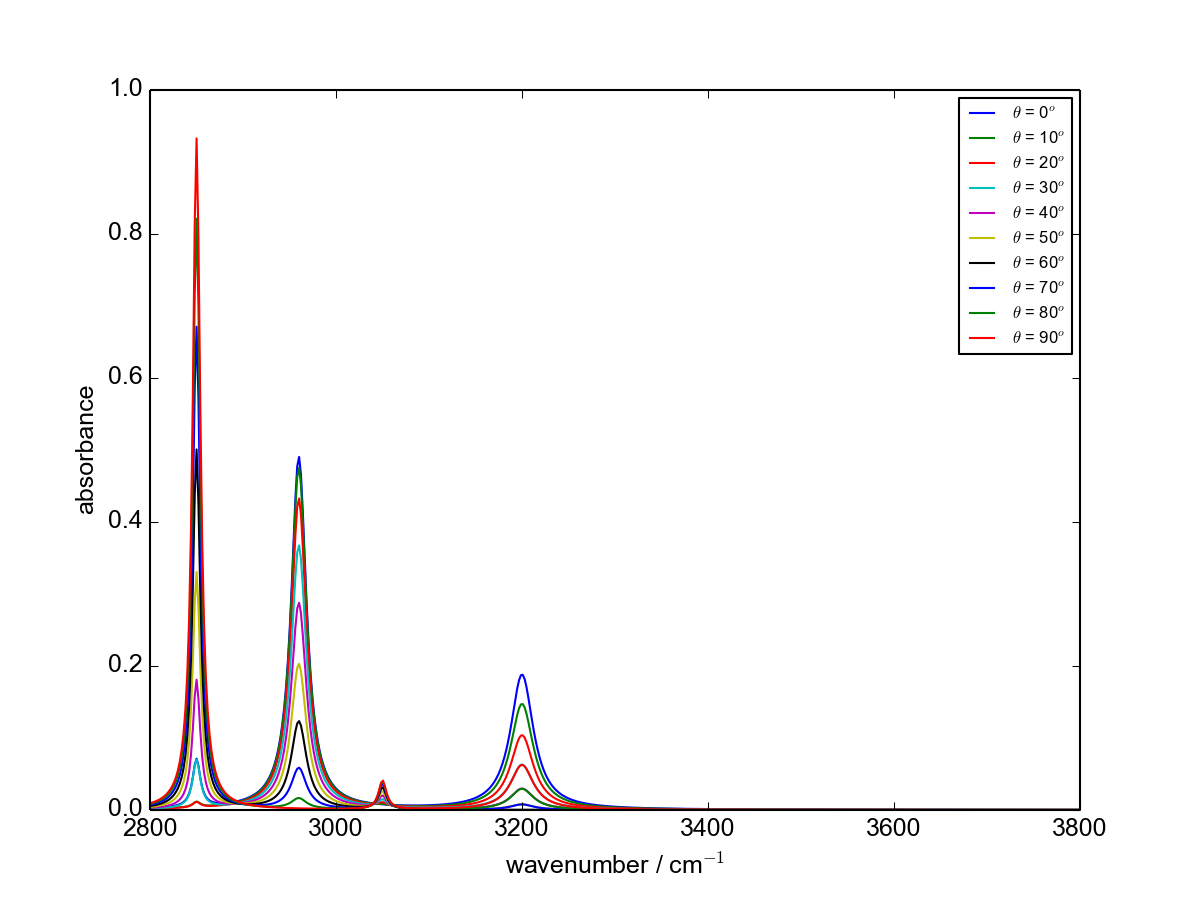
\includegraphics[scale=0.7]{Figures/Toy_Model_IR_Sine_Projection.png} 
\caption{Toy Model Candidates IR Sine Projection} 
\end{figure}

\begin{table} \label{tab:3.3}
\begin{center}
\begin{tabular}{| l | p{5cm} | l |}
\hline
Experiment index & 4 & 5\\
\hline
Number of Candidates & 4 & 10 \\
\hline
Candidates & [0, 5, 10, 15] & [0, 10, 20, 30, 40, 50, 60, 70, 80, 90] \\
\hline
Target Composition & [0.1, 0.5, 0.4, 0] & [0.1, 0, 0.5, 0, 0.4, 0, 0, 0, 0, 0]\\
\hline
Number of Data Points & 100(cos) + 100(sin) & 100(cos) + 100(sin)\\
\hline
Return Composition & [0.1, 0.5, 0.4, 0] & [0.1, 0, 0.5, 0, 0.4, 0, 0, 0, 0, 0] \\
\hline
\end{tabular} 
\caption{Experiment 4 and 5 Setting}
\end{center}
\end{table}		

%We absorbed that the return composition is the same as the target one. Furthermore, we conducted one more experiment set to see if it does help for even a bit more complicated situation. We introduced sine projection of IR spectra to Experiment 3. And without surprise, we have the correct result again.

%And this already has shown us that the more information we can get to build the constraints, the more accurate result we will get.
\section{Constraint Study Based on Experiment 4}

From Experiment 1 to 5, we know having sufficing information in our LP model is the key to obtain the target composition. Having sufficing information means having enough constraints to help LP model converge to a desired result. Moreover, the information is coming from the valuable data points selected along the spectra. This leads us to do a further study on the constraints in order to see how many data points are enough to get the desired composition.\\ 

Base on Experiment 4, experiments about constructing LP model with different data information are conducted in Table \ref{tab:3.4}. Number of Data Points indicates how many data points are selected. Points Selection shows how data points are selected. [2800, 3300, 50] means along wavenumber from 2500 to 3300, every 25 wavenumber. For example, Experiment 6 contains 10 data points from cosine-polarized IR spectrum. Every 50 wavenumber, one data point is selected. Similarly, for Experiment 7, 8, 9, 10, 11, every 25, 20, 15, 10 and 5 wavenumber, one data point is select. From Experiment 12 to 16, data points are selected from both cosine-polarized and sine-polarized IR spectrum. \\

(TODO: rethink: What can we exactly get from the following two tables? Should we include this study?)

\begin{table} \small \label{tab:3.4}
\begin{center}
\begin{tabular}{| l | l | p{3cm} | l |} \hline
	Experiment Index & Number of Data Points & Points Selection & Result \\ \hline
	6 & 10 & [2800, 3300, 50] & [0, 0.796962, 0.103038, 0.1] \\ \hline
	7 & 20 & [2800, 3300, 25] & [0, 0.796962, 0.103038, 0.1] \\ \hline
	8 & 25 & [2800, 3300, 20] & [0, 0.796962, 0.103038, 0.1] \\ \hline
	9 & 32 & [2800, 3300, 15] & [0, 0.796962, 0.103038, 0.1] \\ \hline
	10 & 50 & [2800, 3300, 10] & [0, 0.796962, 0.103038, 0.1] \\ \hline
	11 & 100 & [2800, 3300, 5] & [0, 0.796962, 0.103038, 0.1] \\ \hline
	12 & $100 + 1$ & [2800, 3300, 5], [2800, 3300, 500] & [0, 0.796962, 0.103038, 0.1] \\ \hline
	13 & $100 + 5$ & [2800, 3300, 20], [2800, 3300, 100] & [0, 0.796962, 0.103038, 0.1] \\ \hline
	14 & $100 + 10$ & [2800, 3300, 20], [2800, 3300, 50] & [0, 0.796962, 0.103038, 0.1] \\ \hline
	15 & $100 + 50$ & [2800, 3300, 20], [2800, 3300, 10] & [0.1, 0.5, 0.4, 0] \\ \hline
	16 & $100 + 100$ & [2800, 3300, 20], [2800, 3300, 5] & [0.1, 0.5, 0.4, 0] \\ 
	\hline
\end{tabular} 
\end{center}
\caption{Constraint Study Based on Experiment 4}
\end{table}

One interesting result from Table \ref{tab:3.4} is that: from Experiment 1 to 9, the result composition is the same. Au contrary, from Experiment 10, the return composition gets changed to the target one. Furthermore, if we plot the return composition of [0, 0.796962, 0.103038, 0.1] and the target one [0.1, 0.5, 0.4, 0] in  Picture \ref{fig:3.5}. In this picture, we can see that the spectra generated by these two composition are identical.

\begin{figure}[!ht] \label{fig:3.5}
\centering
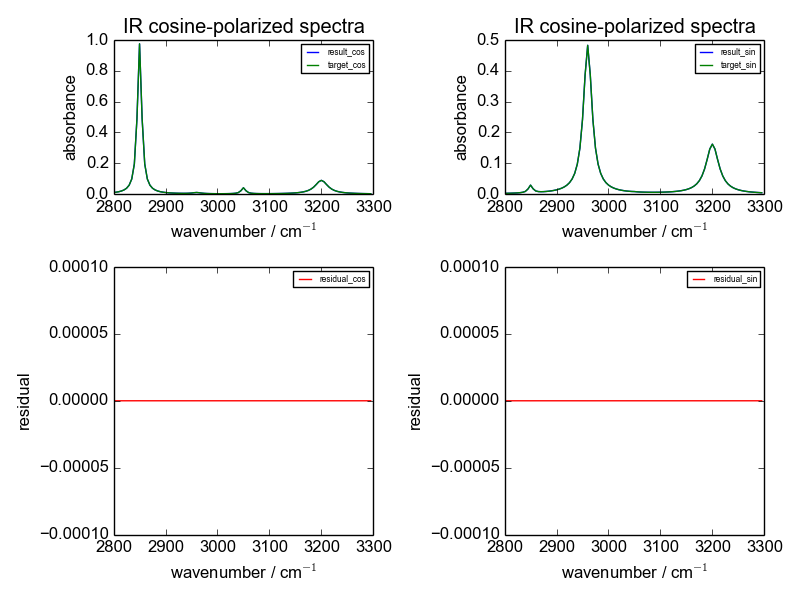
\includegraphics[scale=0.3]{Figures/toy_model_result_plotting_ir_sin_4candi_constraint_study_experiment4.png} 
\caption{Toy Model Constraint Study 1}
\end{figure}


\section{Constraint Study Based on Experiment 5}

And when the same constraint study is applied to the experiments based on Experiment 5 in Table \ref{tab:3.6}, the observation is the same as the experiments in Table \ref{tab:3.4}. This further proves that: We can obtain different solutions by have different constraints. When the  result composition [0, 0, 0.730541, 0, 0.212061,0, 0, 0.0573978, 0, 0] and target one [0.1, 0, 0.5, 0, 0.4, 0, 0, 0, 0, 0] are plotted together, they are almost identical as well, as shown in Picture \ref{fig:3.6}.

\begin{table} \tiny \label{tab:3.6}
\begin{center}
\begin{tabular}{| l | l | p{3cm}  | p{6cm} |}
\hline
Experiment Index & Points & Point Selection & Result \\ \hline
17 & 10 & [2800, 3300, 50] & [0.156758, 0, 0, 0.825977, 0, 0, 0, 0, 0, 0.017265] \\ \hline
18 & 25 & [2800, 3300, 20] & [0, 0, 0.730541, 0, 0.212061, 0, 0, 0.0573978, 0, 0, 0] \\ \hline
19 & 50 & [2800, 3300, 10] & [0, 0, 0.730541, 0, 0.212061, 0, 0, 0.0573978, 0, 0, 0] \\ \hline
20 & 100 & [2800, 3300, 5] & [0, 0, 0.730541, 0, 0.212061, 0, 0, 0.0573978, 0, 0, 0] \\ \hline
21 & 500 & [2800, 3300, 5] & [0, 0, 0.730541, 0, 0.212061, 0, 0, 0.0573978, 0, 0, 0] \\ \hline	
22 & $100 + 1$ & [2800, 3300, 5], [2800, 3300, 500] & [0, 0, 0.730541, 0, 0.212061, 0, 0, 0.0573978, 0, 0, 0] \\ \hline
23 & $100 + 10$ & [2800, 3300, 5], [2800, 3300, 50] & [0.361587, 0, 0.312061, 0.326352, 0, 0, 0, 0, 0] \\ \hline
24 & $100 + 20$ & [2800, 3300, 5], [2800, 3300, 25] & [0.174023, 0, 0, 0.791447, 0, 0, 0.0345301, 0, 0, 0] \\ \hline
25 & $100 + 25$ & [2800, 3300, 20], [2800, 3300, 20] & [0.174023, 0, 0, 0.791447, 0, 0, 0.0345301, 0, 0, 0] \\ \hline
26 & $100 + 50$ & [2800, 3300, 5], [2800, 3300, 10] & [0, 0, 0.753209, 0, 0.146791, 0, 0.1, 0, 0, 0] \\ \hline
27 & $100 + 84$ & [2800, 3300, 5], [2800, 3300, 6] & [0.174023, 0, 0, 0.791447, 0, 0, 0.0345301, 0, 0, 0] \\ \hline
28 & $100 + 100$ & [2800, 3300, 5], [2800, 3300, 5] & [0.1, 0, 0.5, 0, 0.4, 0, 0, 0, 0, 0] \\ 
\hline
\end{tabular} \\
\caption{Constraint Study Based on Experiment 5}
\end{center}
\end{table}

\begin{figure}[!ht] \label{fig:3.6}
\centering
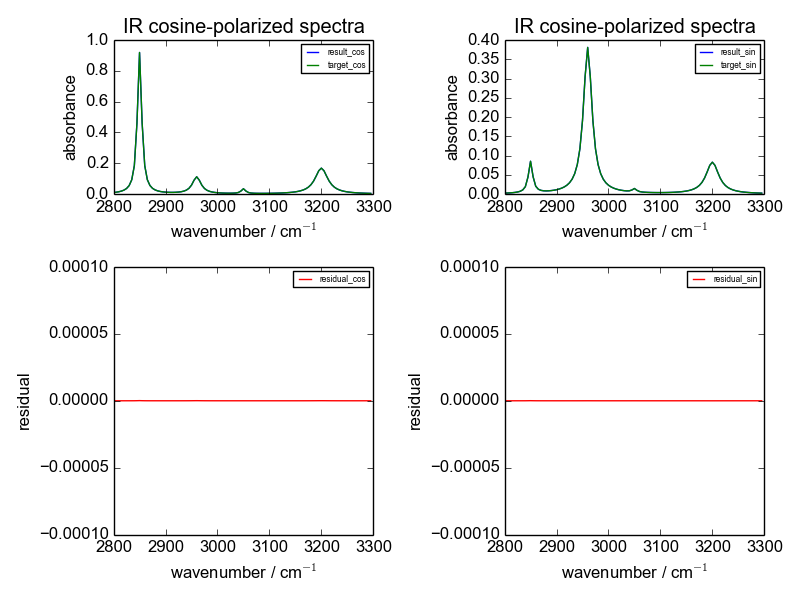
\includegraphics[scale=0.3]{Figures/toy_model_result_plotting_ir_sin_10candi_constraint_study_experiment5.png} 
\caption{Toy Model Constraint Study 2}
\end{figure}

\section{Discussion and Conclusion}
%During the try-out, we first select the data points at the peaks, which are four points at frequency of 2850, 2960, 3050 and 3200. We then construct the Linear Programming model based on these data points. The result returned by LP-solver matched to the known one. However, if we randomly select four data points, the returned result usually does not match to the know one. At the end, we increase the number of data points, at each 5 wavelength frequency gap, a data point will be selected. And the returned result will eventually match to the known one. \\

%The more data points we select, the more information about the candidates and targeted spectrum we will have in our model. Therefore, the more complicated and complete model we will construct. As we select one data point, a new variable is introduced to our model, meanwhile, two new constraints are brought into our model as well. This means that solution space is further and better restricted. When we select data points only on the peaks, these data points already contains enough information for the solver to distinguish the candidates. However, if we randomly select four data points, they may not contain enough information in order to construct the model to obtain the desired result. 

With all the experiments conducted with the toy model, we have learnt that the reason, that LP model does not return a composition that matches to the target one, is the model does not have sufficing information to build the constraints that will converge the result to the target one. However, with the limited information, the optimal solution returned by LP model does build the perfect target spectrum. This means that the solution for the composition that achieve minimum residual of the objective function is not unique ideally. However, in real experiment, because numerical restriction, an unique optimal solution is obtained from the LP model. \\

The above analysis throws a question: how can we know there is enough information to achieve the target composition? In the next step, we will experiment with the real molecules. The goal is to check with all the spectral information we can obtain for real molecules, can our LP model return the target composition for the target spectrum? If yes, can we apply the LP model systematically? Furthermore, to maximally explore the capacity of our LP model, and study its limitation. Finally, come up with some general instructions for applying our LP model. These are the main focus for the following chapters.\\

		

		 



